\section{Reliability Analysis of Water Supply Network} 
    In this section, crude Monte Carlo and importance sampling methods are compared to determine the reliability of a water supply network (WSN) exposed to seismic hazards. Two water distribution networks are considered for this purpose: the first one is a small hypothetical network with only 8 pipelines and the second one is the Charleston water supply network with more than 1800 pipelines located in Charleston, SC.\\
    A water supply network consists of several components, such as pipelines, valves, tanks, and pumps, of which pipelines account for the most capital and rehabilitation costs \cite{kleiner_long-term_1998}. Because they connect supply and demand points, they are also the most important part of a WSN's ability to keep running. Therefore, among all the components of a WSN, the focus of this study is only on pipelines.\\
    Pipelines in a WSN fail based on their probability of failure calculated according to the method presented in the American Lifelines Alliance guidelines \cite{american_lifelines_alliance_ala_seismic_2001, american_lifelines_alliance_ala_seismic_2005}. $P_{fj}$ equals one minus the probability of zero failure, which can be calculated using a Poisson probability distribution of estimated failures or repairs expressed as \cite{fragiadakis_seismic_2014}: 
    $$P_{fj} = 1-e^{RR_j\times L_j}$$
    where $RR_j$ is the repair rate (number of repairs/km/year) of pipeline $j$; and $L_j$ is the length of pipeline $j$ in $km$ $(1 km = 3281 ft)$.\\ 
    The repair rate $(RR)$ of buried pipelines can be calculated based on the type of seismic hazards. Transient ground deformation $(TGD)$ and permanent ground deformation $(PGD)$ are common effects of seismic hazards on buried pipelines. The $TGD$ seismic hazard is the result of ground shaking, while the $PGD$ hazard may be the result of fault displacement, landslides, or liquefaction ground failures. Regression models suggested in \cite{american_lifelines_alliance_ala_seismic_2001} are used to estimate the repair rate $(RR)$ due to $TGD$ and $PGD$ and are expressed as follows:
    $$RR_{TGD}=K_{1}K_{t}\times 0.00241\times PGV$$
    $$RR_{PGD}=K_{2}K_{t}\times 2.58\times PGD^{0.319}$$
    Where $RR_{TGD}$ and $RR_{PGD}$ are the number of estimated repairs per $1 km$ per year of pipeline length due to $TGD$ and $PGD$ hazards, respectively; $PGV$ is peak ground velocity in $cm/sec$ $(1 cm = 0.39 inch)$; $PGD$ is permanent ground deformation in $cm$ $(1 cm = 0.39 inch)$; $K_1$ and $K_2$ are correction factors for pipe size and material as presented in Table~\ref{table:k1&k2}; and $K_t$ is the correction factor for the structural health of the pipeline as presented in Table~\ref{table:kt}. Similar to what was taken into account by \cite{fragiadakis_seismic_2014} and \cite{ball_baltimores_2015}, $K_t$ characterizes the impact of a pipeline's failure history on its failure probability. The deterioration pattern suggested by \cite{fragiadakis_seismic_2014} is used to estimate $K_t$ in this study based on the number of prior failures, with the assumption that a pipeline breakdown will occur 10 years from now.
    The combined repair rate is estimated using the probability of significant liquefaction as follows \cite{american_lifelines_alliance_ala_seismic_2001}: 
    $$RR=(1-P_{Liq})RR_{TGD}+P_{Liq}RR_{PGD}$$
    where $P_{Liq}$ is the probability of liquefaction in percent obtained from a liquefaction potential map.\\ 
    
    \begin{table}[H]
	\centering
	\caption{Coefficients for Adjusting Repair Rate attributable to $TGD$ and $PGD$ (Adapted from \protect \cite{american_lifelines_alliance_ala_seismic_2001})}
	\label{table:k1&k2}
	\small
	\begin{tabular}{lcc}
		\hline
		Pipe Material & $k_1$ & $k_2$\\ \hline
		Cast iron & 1.0 & 1.0 \\
		Welded steel diameter $\geq 406.4mm$ & 0.15 & 0.7 \\
		Welded steel diameter $101.6–304.8 mm$ & 0.7 & 0.7 \\
		Asbestos cement & 1.0 & 1.0 \\
		PVC & 0.5 & 0.8 \\
		Ductile iron & 0.5 & 0.5 \\
		\hline
	\end{tabular}
\end{table}
    \begin{table}[H]
	\centering
	\caption{Coefficient for Adjusting the Repair Rate Based on Pipeline Condition}
	\label{table:kt}
	\small
	\begin{tabular}{lc}
		\hline
		Number of Previous Breaks & $k_t$\\ \hline
		0 & 1 \\
		1-4 & 2 \\
		5-8 & 8 \\
		$\geq 8$ & 37 \\
		\hline
	\end{tabular}
\end{table}
    
    Upon estimating the failure probability of each pipeline, their failure status is determined according to the sampling methods, each of which will be discussed separately later. In a damaged WSN, the failed pipelines are represented by leaks or breaks that exist there. The total number of leaks/breaks in the failed pipelines can be generated as a Poisson random number with the mean arrival rate equal to the estimated repair rate ($RR$) \cite{hwang_seismic_1998} which then will be divided into the number of leaks (NLKS) and the number of breaks (NBKS) according to the pipe material and the type of seismic hazard \cite{hwang_seismic_1998}.\\ 
    According to \cite{ballantyne_earthquake_1991}, 15\% of cast iron pipes (CIP) will break and 85\% of them will leak as a result of TGD hazards. Similarly, due to the TGD hazard, 96\% of ductile iron pipes (DIP) will leak and 4\% will break. Additionally, it is reported that 50\% of all pipe materials will leak and 50\% will break due to PGD hazards. These empirical results are used to calculate the total number of leaks and breaks using the following equations: 
    $$N_{LKS}=LKS_{TGD}+LKS_{PGD}$$
    $$N_{BKS}=BKS_{TGD}+BKS_{PGD}$$
    where $N_{LKS}$ and $N_{BKS}$ are the total numbers of leaks and breaks in each pipeline, respectively; $LKS_{TGD}$ and $BKS_{TGD}$ are the total numbers of leaks and beaks due to $TGD$, respectively; and $LKS_{PGD}$ and $BKS_{PGD}$ are the total numbers of leaks and beaks due to $PGD$, respectively. \\ 
    After estimating the number of leaks and breaks in the failed pipelines, the damaged WSN is simulated using an open-source Python™ package called Water Network Tool for Resilience (WNTR) \cite{klise_water_2017} which uses a pressure-driven demand (PDD) approach to evaluate the ability of a damaged WSN to meet the system demand. In this approach, leaks and breaks are simulated by adding an orifice in the middle of the failed pipeline. The orifice area in this study is considered to be $3\%$ of the pipeline cross-sectional area for a leak and $20\%$ for a break \cite{hwang_seismic_1998}. Then, the following equation is used to figure out the total orifice area of a failed pipeline: 
    $$ A_T=(0.03 N_{LKS}+0.2 N_{BKS}) \times A $$
    where $A_T$ is total orifice area of the damaged pipeline in $mm^2$ $(1 mm^2 = 0.0015 in^2)$; $A$ is pipeline cross-sectional area in $mm^2$. The upper bound of $A_T$ is assumed to be one cross-sectional area of the pipeline. \\
    Finally, system reliability is defined as the average ratio of satisfied demand to required demand for all demand nodes in the WSN.
    % To do this, an inverse normal CDF of a pipeline's failure probability with a mean value of 0 and a standard deviation of 1 will be compared to a multivariate normal number with a mean value of 0 and a covariance of a diagonal matrix of 1. 

    % Upon estimating the probability of failure of each pipeline, the damaged WSN is simulated using a pressure-driven demand (PDD) approach to evaluate its ability to meet the system demand. In the damaged WSN, pipelines are randomly failed based on their failure probability and 
    
    \subsection{Small Water Supply Network}
        The simplified two-loop water supply network used to compare the crude Monte Carlo with the Importance Sampling technique is shown in Fig.~\ref{fig:Small_WSN}. This network is derived from the \textit{Alperovits and Shamir} problem \cite{alperovits_design_1977} for which nodal head and demands are given as in Table~\ref{table:small_WSN_nodes} and all pipes 1000 $m$ long. The pipeline's characteristics and hazard information are assumed as presented in Table~\ref{table:small_WSN_edges}. Also, the $PGV$ for the entire network is assumed to be 49.5 $cm/s$.% which is based on a $PGA$ of $0.3g$.
            
                \begin{figure}[H]
        \centering
        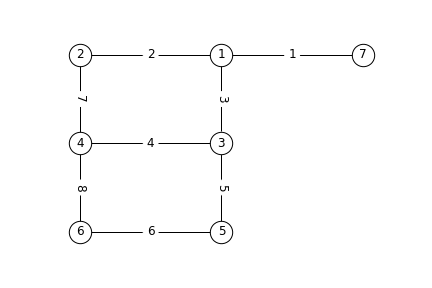
\includegraphics[scale=0.50]{Figures/Images/Reliability Analysis of Water Supply Network/small_WSN.png}
        \caption{The layout of the small water supply network}
        \label{fig:Small_WSN}
    \end{figure}
            \begin{table}[H]
	\centering
	\caption{Head and demand values for the small water supply network}
	\label{table:small_WSN_nodes}
	\small
	\begin{tabular}{ccc}
    	\hline
    	\textbf{Node ID} & \Centerstack{\textbf{Head} \\ $(m)$} & \Centerstack{\textbf{Demand} \\ $(m^3/h)$} \\ 
            \hline
    	\textbf{1} & 210 & -1120.0 \\
    	\textbf{2} & 150 & 100 \\
    	\textbf{3} & 160 & 100 \\
    	\textbf{4} & 155 & 120 \\
            \textbf{5} & 150 & 270 \\
            \textbf{6} & 165 & 330 \\
            \textbf{7} & 160 & 200 \\
    	\hline
	\end{tabular}
\end{table}
            \begin{table}[H]
	\centering
	\caption{Pipeline charachteristics and hazard information for the small water supply network}
	\label{table:small_WSN_edges}
	\small
        \strutlongstacks{T}
	\begin{tabular}{cccccc}
    	\hline
    	\textbf{Link ID} & \Centerstack{\textbf{Diameter} \\ $(cm)$} & \textbf{Material} & \textbf{LPI$^a$} & \textbf{NOPB$^b$} & \Centerstack{\textbf{PGD} \\ $(cm)$}\\ 
            \hline
    	\textbf{1} & 55.9 & DIP & 0.35 & 0 & 0.516\\
    	\textbf{2} & 30.5 & DIP & 0.65 & 0 & 1.716\\
    	\textbf{3} & 35.6 & DIP & 0.65 & 0 & 1.716\\
    	\textbf{4} & 15.2 & DIP & 0.75 & 0 & 1.016\\
            \textbf{5} & 35.6 & DIP & 0.65 & 1 & 1.016\\
            \textbf{6} & 35.6 & DIP & 0.85 & 0 & 1.916\\
            \textbf{7} & 35.6 & DIP & 0.65 & 1 & 1.716\\
            \textbf{8} & 25.4 & DIP & 0.85 & 0 & 1.716\\
    	\hline
            \multicolumn{2}{l}{\footnotesize $^a$ Liquefaction Potential Index} \\
            \multicolumn{2}{l}{\footnotesize $^b$ Number of Previous Breaks}
	\end{tabular}
\end{table}

        As previously stated, the goal here is to estimate the reliability of the WSN given known hazards and pipeline characteristics. After estimating the failure probability and the number of leaks and breaks for each pipeline, and since the small WSN has only 8 pipelines, the actual expected value for the network's reliability can be calculated. However, even for a small WSN with only 8 pipelines, it would take a long time to find the near-optimal importance density function using the traditional trial-and-error method. Consequently, only the crude Monte Carlo and MCMC-IS methods are compared for estimating the reliability of the small WSN. For MCMC-IS, both regular and adaptive techniques to generate MCMC samples are examined, and the results are presented in Table~\ref{table:small_WSN_results}. 
        
            \begin{table}[H]
    \centering
    \caption{Comparison of the estimation, variance, and MSE produced by the three estimators with the sample size of 10 for the small WSN}
    \label{table:small_WSN_results}
    \small
    \begin{tabular}{lccc}
        \hline
        & \textbf{crude MC} & \textbf{Regular MCMC-IS} & \textbf{Adaptive MCMC-IS} \\
        \hline
        \textbf{Estimation}\\
        true value = 0.0629 & 6.351e-2 & 7.257e-2 & 7.655e-2\\
        \textbf{Variance} & 9.440e-4 & 1.932e-5 & 1.706e-4\\
        \textbf{Mean Square Error (MSE)} & 9.444e-4 & 1.133e-4 & 3.576e-4\\
        \hline
    \end{tabular}
\end{table}
            
    \subsection{Large Water Supply Network}
        In this section data for the WSN in the Charleston peninsula region in South Carolina are used to compare the performance of crude Monte Carlo and Importance Sampling techniques. The layout of the Charleston water supply network (CWSN), is depicted in Fig.~\ref{fig:CWSN}. CWSN is a massive network covering an area of eight square miles of land, with a distribution pipeline length of around 150 km (1 km = 0.62 miles), to service about 33,971 consumers \cite{noauthor_city_2021}. \\
        CWSN consists of 1,874 individual pipeline links and 1,474 demand nodes. CWSN pipelines range in diameters from 25.4 to 609.6 mm (1 mm = 0.039 in.) where the majority of them (57.3\%) have diameters less than 152 mm and are made of different materials (22.4\% cast iron pipe–CIP; 69.2\% ductile iron pipe—DIP; and 8.4\% the Other category that includes polyvinyl chloride and galvanized steel).
        Information on CWSN pipeline failures in the past is used to assess the system's present state of health. There have been 315 recorded pipeline failures, according to failure data during a roughly 10-year period (2002–2012).

                \begin{figure}[H]
        \centering
        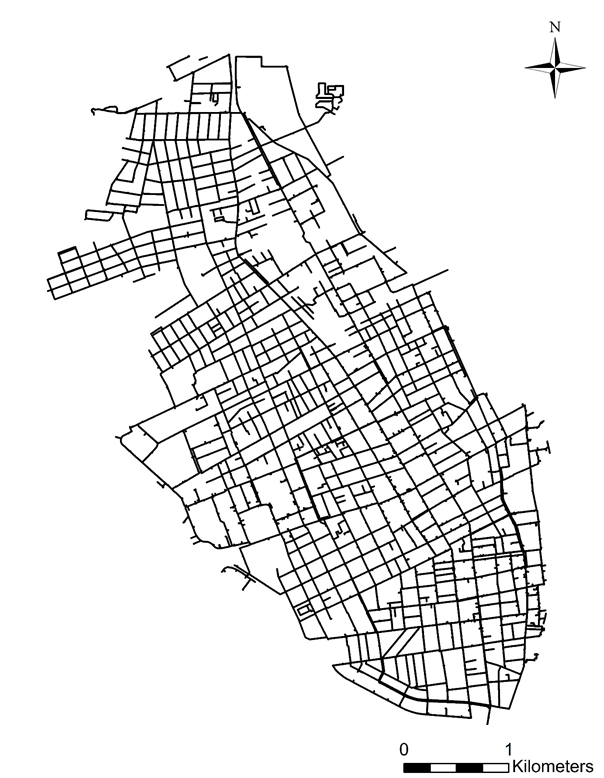
\includegraphics[scale=0.5]{Figures/Images/Reliability Analysis of Water Supply Network/CWSN.png}
        \caption{The layout of the Charleston water supply network}
        \label{fig:CWSN}
    \end{figure}

        Charleston is vulnerable to both TGD and PGD hazards. In August 1886, an earthquake with an MW of $\sim7$ centered approximately 30 $km$ northeast of the Charleston peninsula caused major damage throughout the region resulting in 124 deaths and \$540 million
        (2014 dollars) in damages (Côté 2006). PGD failures on the peninsula were common (Dutton 1889; Robinson and Talwani 1983; Hayati and Andrus 2008).
        Hayati and Andrus (2008) compiled available geotechnical field test information and applied the liquefaction potential index (LPI) approach, originally proposed by Iwasaki et al. (1978), to
        develop the geology-based liquefaction potential map presented
        in Fig.~\ref{fig:CWSN_LPI}, assuming the peak ground acceleration (PGA) of 0.3 g.
        Detailed information on how to develop LPI for CWSN can be found in.
        Concerning TGD, it is calculated using a PGV of 49.5 cm/s.
        This estimate of PGV is based on a PGA of 0.3 g and various empirical relationships (Wald et al. 1999; Kaka and Atkinson 2004;
        Campbell and Bozorgnia 2008; Wu et al. 2003).

                \begin{figure}[H]
        \centering
        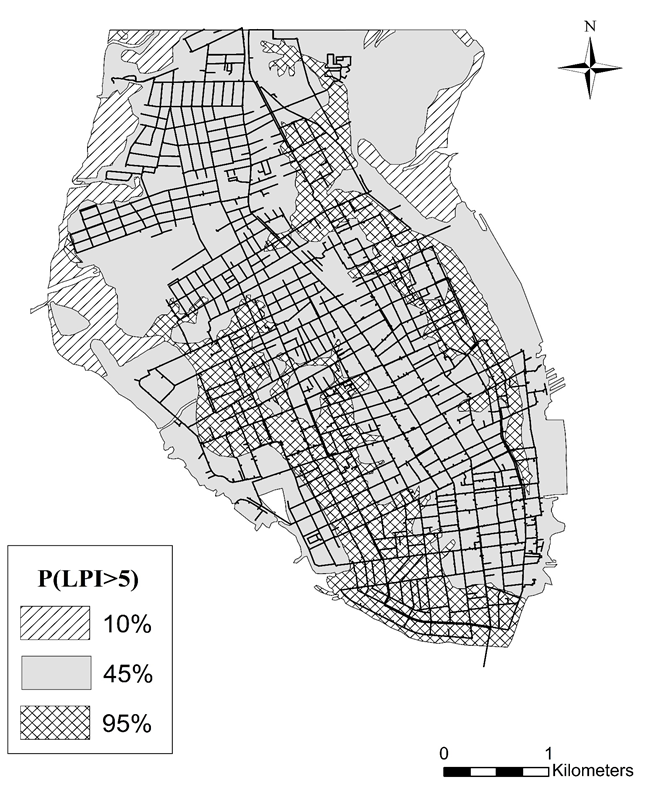
\includegraphics[scale=0.5]{Figures/Images/Reliability Analysis of Water Supply Network/CWSN_LPI.png}
        \caption{Liquefaction potential map of the Charleston peninsula with the CWSN overlaid}
        \label{fig:CWSN_LPI}
    \end{figure}
    


